
%(BEGIN_QUESTION)
% Copyright 2015, Tony R. Kuphaldt, released under the Creative Commons Attribution License (v 1.0)
% This means you may do almost anything with this work of mine, so long as you give me proper credit

There are several different methods of providing {\it reduced-voltage starting} for electric motors.  One of them is the {\it autotransformer} method.  Here is a diagram showing how this works:

$$\includegraphics[width=15.5cm]{i02309x01.eps}$$

``L1,'' ``L2,'' and ``L3'' represent the three phase power supply conductors.  Three sets of contacts (R, S, and Y) serve to connect power to the motor at different times.  The starting sequence for the motor is as follows:

\begin{itemize}
\item{1.} Motor off (R open, S open, Y open) 
\item{2.} Start button pressed (S and Y contacts all close)
\item{3.} Time delay (depending on the size of the motor)
\item{4.} Y contacts open
\item{5.} Time delay (depending on the size of the motor)
\item{6.} R contacts close, S contacts open
\end{itemize}

Explain the operation of this system.  How do the autotransformers serve to reduce voltage to the electric motor during start-up?

\vskip 20pt \vbox{\hrule \hbox{\strut \vrule{} {\bf Suggestions for Socratic discussion} \vrule} \hrule}

\begin{itemize}
\item{} A problem-solving technique useful for analyzing circuits is to {\it re-draw the circuit} in a form that is easier to follow than what is shown to you on the given diagram.  Discuss and compare different renderings of this circuit, and how these simplified sketches help you with the analysis.
\item{} Explain the purpose of the devices labeled ``CT'' in this diagram, and also how the overload heaters adequately function even though they are not in series with the motor conductors.
\item{} Explain how the start-up sequence for this electric motor could be controlled by a PLC.
\end{itemize}

\underbar{file i02309}
%(END_QUESTION)





%(BEGIN_ANSWER)

When the ``S'' and ``Y'' contacts are all closed, the autotransformers form a three-phase ``Y'' connection, with line voltage (L1, L2, and L3) applied to the ``tips'' of the ``Y,'' and a reduced motor voltage tapped off a portion of each autotransformer winding.

\vskip 10pt

When the ``Y'' contacts open, the three autotransformers now function merely as series-connected inductors, limiting current with their inductive reactance.

\vskip 10pt

When the ``R'' contacts close, the motor receives direct power from L1, L2, and L3.

\vskip 10pt

Here is a {\it single-phase equivalent} circuit, representing the motor as a resistive load:

$$\includegraphics[width=15.5cm]{i02309x02.eps}$$

%(END_ANSWER)





%(BEGIN_NOTES)

For each step of the start-up sequence, it is possible to re-draw the circuit feeding power to the motor, in order to make its function more apparent.  Do not create these re-drawings yourself, but have your students draw an equivalent circuit for each step in the start-up sequence.


\vskip 20pt \vbox{\hrule \hbox{\strut \vrule{} {\bf Virtual Troubleshooting} \vrule} \hrule}

This question is a good candidate for a ``Virtual Troubleshooting'' exercise.  Presenting the diagram to students, you first imagine in your own mind a particular fault in the system.  Then, you present one or more symptoms of that fault (something noticeable by an operator or other user of the system).  Students then propose various diagnostic tests to perform on this system to identify the nature and location of the fault, as though they were technicians trying to troubleshoot the problem.  Your job is to tell them what the result(s) would be for each of the proposed diagnostic tests, documenting those results where all the students can see.

During and after the exercise, it is good to ask students follow-up questions such as:

\begin{itemize}
\item{} What does the result of the last diagnostic test tell you about the fault?
\item{} Suppose the results of the last diagnostic test were different.  What then would that result tell you about the fault?
\item{} Is the last diagnostic test the best one we could do?
\item{} What would be the ideal order of tests, to diagnose the problem in as few steps as possible?
\end{itemize}

%INDEX% Electronics review: AC motor control circuit

%(END_NOTES)


